\documentclass[tikz,border=3mm,multi=tikzpicture]{standalone}
\usepackage{tikz}
\usetikzlibrary{arrows.meta,calc,positioning}
\begin{document}

% TikZ 1
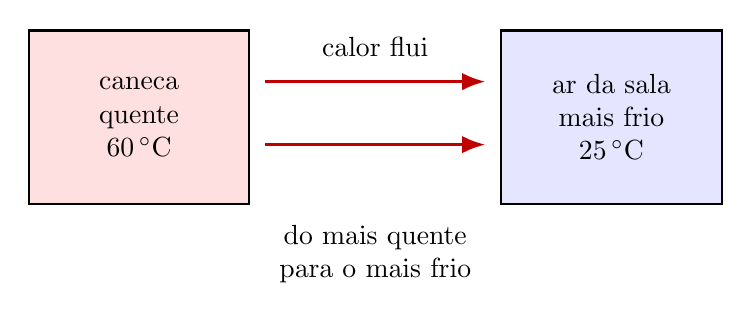
\begin{tikzpicture}[>=Latex]
  \draw[thick,fill=red!12] (0,0) rectangle (2.8,2.2);
  \node[align=center] at (1.4,1.1) {caneca\\quente\\$60\,^{\circ}\mathrm{C}$};
  \draw[thick,fill=blue!10] (6,0) rectangle (8.8,2.2);
  \node[align=center] at (7.4,1.1) {ar da sala\\mais frio\\$25\,^{\circ}\mathrm{C}$};
  \draw[very thick,red!75!black,->] (3.0,1.55) -- (5.8,1.55);
  \draw[very thick,red!75!black,->] (3.0,0.75) -- (5.8,0.75);
  \node[align=center,above] at (4.4,1.75) {calor flui};
  \node[align=center,below] at (4.4,-0.15) {do mais quente\\para o mais frio};
\end{tikzpicture}

% TikZ 2
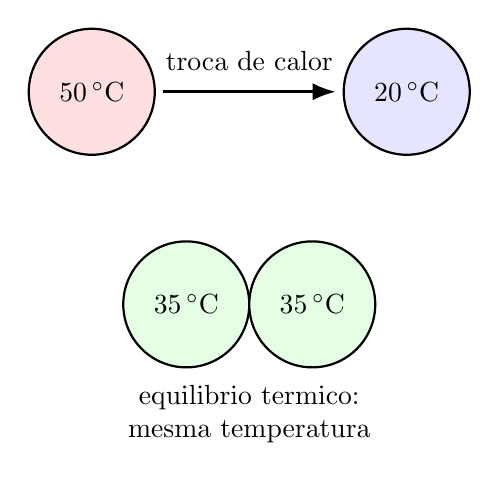
\begin{tikzpicture}[>=Latex]
  \draw[thick,fill=red!12] (0,1.5) circle (0.8);
  \node[align=center] at (0,1.5) {$50\,^{\circ}\mathrm{C}$};
  \draw[thick,fill=blue!10] (4,1.5) circle (0.8);
  \node[align=center] at (4,1.5) {$20\,^{\circ}\mathrm{C}$};
  \draw[very thick,->] (0.9,1.5) -- (3.1,1.5);
  \node[above] at (2,1.65) {troca de calor};

  \draw[thick,fill=green!10] (1.2,-1.2) circle (0.8);
  \draw[thick,fill=green!10] (2.8,-1.2) circle (0.8);
  \node[align=center] at (1.2,-1.2) {$35\,^{\circ}\mathrm{C}$};
  \node[align=center] at (2.8,-1.2) {$35\,^{\circ}\mathrm{C}$};
  \draw[very thick,gray!70] (2.0,-1.2) -- (2.0,-1.2);
  \node[align=center,below] at (2,-2.1) {equilibrio termico:\\mesma temperatura};
\end{tikzpicture}

\end{document}
